
\documentclass{beamer}
\usetheme{Madrid}

\usepackage{amsmath, amssymb, amsthm}
\usepackage{graphicx}
\usepackage{listings}
\usepackage{gensymb}
\usepackage{minted}
\usemintedstyle{friendly}
\definecolor{bg}{rgb}{0.95,0.95,0.95}
\usepackage[utf8]{inputenc}
\usepackage{hyperref}
\newcommand{\nCr}[2]{\,^{#1}C_{#2}}
\usepackage{gvv}\begin{document}

\title{11.16.2.2.1}
\author{EE24BTECH11020 \\ Ellanti Rohith }
\date{\today}
\frame{\titlepage}

\begin{frame}
\frametitle{Question}
 A die is thrown. Find the probability of that the outcome is less than 7.\\ \end{frame}

\begin{frame}
\frametitle{Solution Outline}
\begin{enumerate}
	\item Define a random variable.
	\item Devise the PMF and CDF of the random variable.
	\item Deduce the required probability from the CDF expression.
\end{enumerate}
\end{frame}

\begin{frame}
\frametitle{Variables Used : }
\begin{center}
\begin{tabular}{|c|c|c|}
\hline 
\textbf{Variable name} & \textbf{Description} \\
\hline 
$\vec{S}$ & Sample space \\
\hline 
$\vec{X}$ & Random variable corresponding to the number on die\\
\hline

$F_{\vec{X}} (x)$ & Cumulative distribution function ( CDF ) \\
\hline
$p_{\vec{X}} (x)$ & Probability Mass function ( PMF ) \\
\hline
\end{tabular}
\end{center}
\end{frame}

\begin{frame}
	
Each outcome is equally likely.

Let \( X \) be the number obtained when the die is rolled.

\[
X \in S
\]
\begin{center}
\begin{tabular}{|c|c|c|}
\hline 
\textbf{Event} & \textbf{Sample space} \\
\hline
$p_{\vec{X}} (1)$ & \cbrak{1} \\
\hline
$p_{\vec{X}} (2)$ & \cbrak{2} \\
\hline
$p_{\vec{X}} (3)$ & \cbrak{3} \\
\hline
$p_{\vec{X}} (4)$ & \cbrak{4} \\
\hline
$p_{\vec{X}} (5)$ & \cbrak{5} \\
\hline
$p_{\vec{X}} (6)$ & \cbrak{6} \\
\hline
\end{tabular}
\end{center}

Since the die is fair, each outcome has an equal probability:

\[
p_X(k) =
\begin{cases}
\frac{1}{6}, & k \in \{1,2,3,4,5,6\} \\
0, & \text{otherwise}
\end{cases}
\]
\end{frame}
\begin{frame}
\frametitle{CDF}

By the definition of the cumulative distribution function (CDF):

\[
F_X(k) = P(X \leq k) = \sum_{i=-\infty}^{k} p_X(i)
\]

Thus, the CDF is given by:

\[
F_X(k) =
\begin{cases}
0, & k < 1 \\
\frac{1}{6}, & 1 \leq k < 2 \\
\frac{2}{6}, & 2 \leq k < 3 \\
\frac{3}{6}, & 3 \leq k < 4 \\
\frac{4}{6}, & 4 \leq k < 5 \\
\frac{5}{6}, & 5 \leq k < 6 \\
1 & k \geq 6
\end{cases}
\]
\end{frame}
\begin{frame}
We need to find:
\[
P(X < 7) = P(X \leq 6) = \sum_{i=1}^{6} P(X = i)\\
= \frac{1}{6} + \frac{1}{6} + \frac{1}{6} + \frac{1}{6} + \frac{1}{6} + \frac{1}{6}
\]

\[
= \frac{6}{6} = 1
\]

Thus,
\[
P(X < 7) = 1
\]
\end{frame}




\begin{frame}
\frametitle{Simulation}
\begin{enumerate}
	\item Generate a random number  using the \textbf{rand()} function. 
	\item Restrict  random numbers from $1$ to  $6$ by using rand() \% 6 operator.
	\item Count the number of favourable outcomes by iterating for a large number of trails.
	\item Divide it by the total number of trails to get the desired PMF.
	\item CDF can then be simulated by summing the required PMFs.
\end{enumerate}
\end{frame}

\begin{frame}
\frametitle{PMF - Plot}
\begin{figure}[h]
\centering
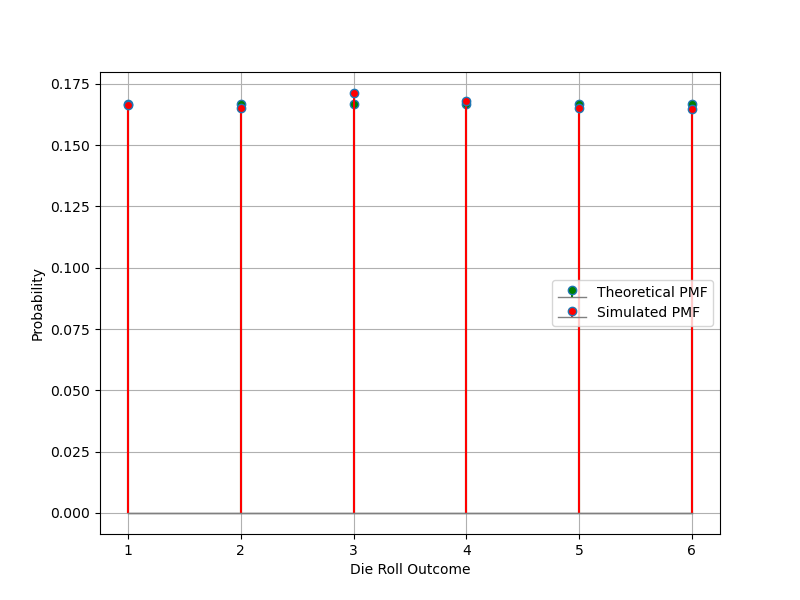
\includegraphics[width=\textwidth]{Figs/Figure_1 (1).png}
\caption{Probability Mass Function}
\label{fig:Plot1} 
\end{figure}
\end{frame}

\begin{frame}
\frametitle{CDF - Plot}
\begin{figure}[h]
\centering
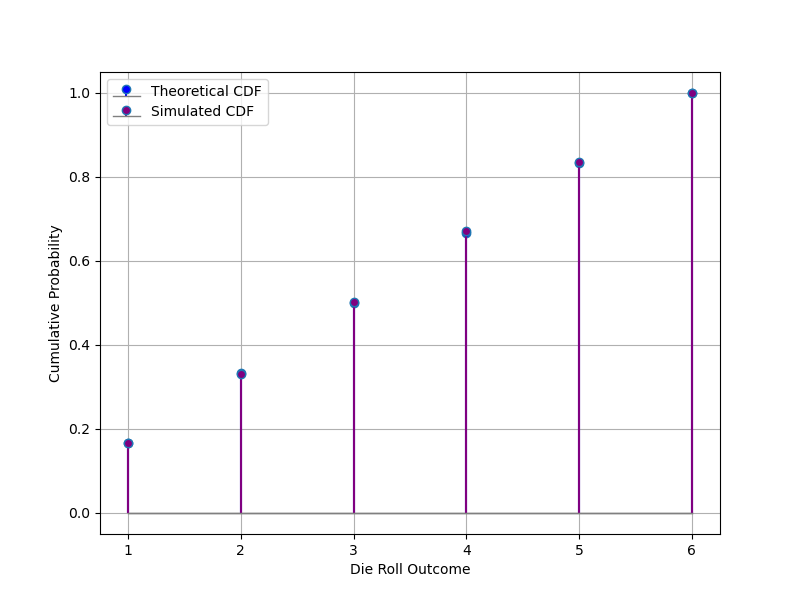
\includegraphics[width=\textwidth]{Figs/Figure_2.png}
\caption{Cumulative Distribution Function}
\label{fig:Plot2} 
\end{figure}
\end{frame}
\end{document}
